\documentclass[12pt]{article}
\usepackage[spanish,mexico]{babel}
	\selectlanguage{spanish}
\usepackage{graphicx}
\usepackage{amsmath}
\usepackage{wrapfig}
\usepackage{float}
\usepackage{multicol}
\usepackage{geometry}
\usepackage{hyperref}
\usepackage[utf8]{inputenc}

\newgeometry{top=3cm}

\title{Actividad 6: Período del péndulo}
\author{Ana Gabriela Carretas Talamante}
\date{01 de marzo de 2016}

\begin{document}
\maketitle
\section{Introducción}
Anteriormente hablamos sobre la ecuación diferencial que describe el movimiento del péndulo y la resolvimos utilizando una librería especial de Python con condiciones de ángulos pequeños. En esta ocasión trabajaremos con la integral que muestra sobre el período del péndulo, haciendo variar el ángulo inicial sin esa restricción. \\

\begin{multicols}{2}
Podemos calcular el período exacto invirtiendo la ecuación de velocidad angular:
\begin{eqnarray}
\frac{d\theta}{dt}=\sqrt{\frac{2g}{l}(\cos{\theta}-\cos{\theta_0})} \\
\frac{dt}{d\theta}=\sqrt{\frac{l}{2g}}\frac{1}{\sqrt{(\cos{\theta}-\cos{\theta_0})}}
\end{eqnarray}
Y luego integrando 4 veces un cuarto de ciclo, lo que nos dejaría la integral a resolver:
\begin{equation}
\label{T}
T=4\sqrt{\frac{l}{2g}}\int_0^{\theta_0}\frac{1}{\sqrt{(\cos{\theta}-\cos{\theta_0})}}
\end{equation}

Encontramos el error relativo al dividir el resultado de \eqref{T} entre el período inicial:
\begin{equation}
\label{T0}
T_0=2\pi\sqrt{\frac{l}{g}}
\end{equation}

\begin{figure}[H]
\centering
\includegraphics[width=8cm]{00}
\caption{Desviación entre el período real y el calculado con la aproximación de ángulos pequeños mientras $\theta_0$ aumenta \cite{W}.}
\end{figure}
\end{multicols}

\begin{figure}[H]
\centering
\includegraphics[width=12cm]{0}
\caption{Valores de desviación entre el período real y el calculado con la aproximación de ángulos pequeños mientras $\theta_0$ aumenta \cite{P}. }
\end{figure}

Mientras el valor de $\theta_0$ crezca hasta acercarse a valores donde $\theta_0 \sim \pi$, los resultados del valor relativo del período divergen a $\infty$, como se muestra en las figuras 1 y 2. \\

El método \textit{scipy.integrate.quad} \cite{S1} nos ayuda a resolver integrales con la librería  QUADPACK de Fortran. Este trabaja analizando la pendiente de la función que va a integrar, relacionándola con el intervalo que va a utilizar para la integración numérica para maximizar la eficiencia del cálculo \cite{SO}.

\subparagraph*{Programa: Resolviendo la integral para el período del péndulo}

Se presenta a continuación el código realizado, donde variamos el ángulo inicial desde un error $e$ hasta el ángulo $\pi+e$. Esto se hizo para evitar que tuviera una integral con 0 en el cociente \cite{M}. Utilizando el método para integrar de \textit{scipy.integrate.quad}, se pudo calcular el valor del período para cada valor de $\theta_0$ indicado por el array ya definido. Al finalizar estos cálculos, se obtuvo el error relativo entre el período calculado y el inicial, y con esto se graficó a $\displaystyle \theta_0 \quad \text{vs} \quad \frac{T}{T_0}$.

\begin{verbatim}
#Bibliotecas utilizadas
from scipy.integrate import quad
import numpy as np
import matplotlib.pyplot as plt

#------------------------------------------
#Definimos las constantes 
#Valor de la gravedad
g=9.8        
#Longitud de la cuerda
l=0.5          
#Periodo inicial
T0=2*np.pi*np.sqrt(l/g)
#Constante de la integral para angulos pequeños
k=4*np.sqrt(l/(2*g))

#------------------------------------------
#Defino los posibles angulos para integrar
n=100
#Error añadido para que no divida entre 0
e=0.0001
#Rango de theta0 
theta00=np.linspace(e,(np.pi)+e,n) 

#------------------------------------------
#Defino los arrays para todos los resultados arrojados
II=[0 for i in range(n)]
err=[0 for i in range(n)]
T=[0 for i in range(n)]

#------------------------------------------
#Definiendo la integral
def I(x, theta0):
    return 1/np.sqrt(np.cos(x)-np.cos(theta0))

#Comienzo un loop para poder calcular todos los resultados 
#posibles contemplando un angulo inicial variante
for i in range(n):
    theta0=theta00[i]
    II[i] , err[i]=quad(I, 0, theta0, args=(theta0))
    T[i]=k*II[i]

#Calulo el periodo real entre el
#periodo calculado y el inicial
real=T/T0

#------------------------------------------    
#Para la grafica
plt.plot(theta00, real, "mo", theta00, real, "g")
plt.title("Desviacion del periodo real con respecto al angulo")
plt.grid()
plt.xlabel("Angulo en radianes")
plt.ylabel("Periodo real")
\end{verbatim}

\subsection*{Analizando las gráficas}
\begin{figure}[H]
\centering
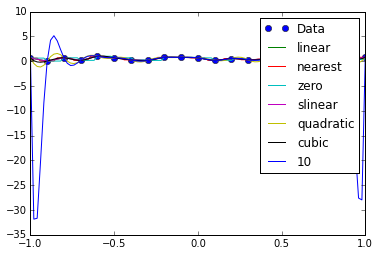
\includegraphics[width=10cm]{1}
\caption{Gráfica generada para n=100.}
\end{figure}

Podemos notar que mientras aumento el tamaño de las particiones del intervalo $(0,\pi)$, el error relativo tiende a $\infty$, como se había mencionado antes.

\begin{figure}[H]
\centering
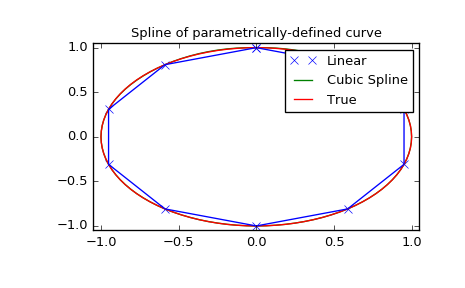
\includegraphics[width=10cm]{2}
\caption{Gráfica generada para n=1000.}
\end{figure}

\begin{figure}[H]
\centering
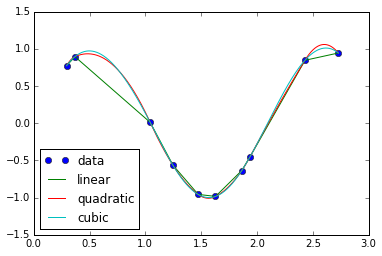
\includegraphics[width=10cm]{3}
\caption{Gráfica generada para n=1500.}
\end{figure}

\begin{figure}[H]
\centering
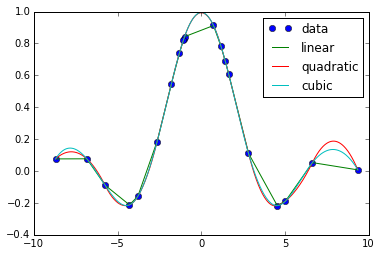
\includegraphics[width=10cm]{4}
\caption{Gráfica generada para n=2000.}
\end{figure}

\pagebreak

\begin{thebibliography}{6}

\bibitem{W}
Alessio Damato,
\emph{Pendulum period}. Recuperado en marzo de 2016 de \url{https://en.wikipedia.org/wiki/Pendulum_\%28mathematics\%29\#/media/File:Pendulum_period.svg}

\bibitem{P}
Algarabia,
\emph{Pendulo Simple - Tabla exacta}. Recuperado en marzo de 2016 de \url{https://commons.wikimedia.org/wiki/File:Moglfm13t02_pendolo_simple_exacto.jpg}

\bibitem{S1}
Scipy,
\emph{quad}. Recuperado en febrero de 2016 de \url{http://docs.scipy.org/doc/scipy/reference/generated/scipy.integrate.quad.html#scipy.integrate.quad}

\bibitem{SO}
Stackoverflow,
Recuperado en marzo de 2016 de \url{http://goo.gl/OOKoYY}

\bibitem{M}
Paredes M., \emph{Asesoría sobre el código}, consultado en febrero de 2016.

\bibitem{FC}
Lizárraga, C.
\emph{Actividad 6 (2016-1)}. Recuperado en febrero de 2016 de \url{http://computacional1.pbworks.com/w/page/105233358/Actividad\%205\%20(2016-1)}

\end{thebibliography}

\end{document}

